% dibuix_cilindre_1.tex
\documentclass{standalone}
\usepackage{tikz}
\usetikzlibrary{arrows.meta, decorations.markings}

\begin{document}

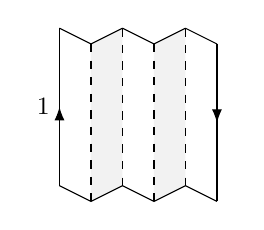
\begin{tikzpicture}[
    identified_edge/.style={
        decoration={
            markings,
            mark=at position 0.5 with {\arrow{Latex}}
        },
        postaction={decorate}
    },
    edge_label/.style={midway, auto, font=\small}
]

\def\squaresize{2}
\def\dentsize{0.2}
% \fill[gray!10] (0,0) -- (0,\squaresize) -- (\squaresize, \squaresize) -- (\squaresize,0) -- cycle;
% \draw (0,0) rectangle (\squaresize,\squaresize);
% \draw[black] (0,\squaresize) -- node[edge_label, above] {} (\squaresize,\squaresize);
% \draw[black] (0,0)       -- node[edge_label, below]  {$\lambda$} (\squaresize,0);

% Draw 5 triangles along the top edge
\foreach \x in {0,0.8} {
    \fill[gray!10] (\x + 0.4,\squaresize - \dentsize) -- (\x + 0.4,-\dentsize) -- (\x + 0.8,0) -- (\x + 0.8,\squaresize) -- cycle;
    \draw (\x,\squaresize) -- (\x + 0.4,\squaresize - \dentsize) -- (\x + 0.8,\squaresize);
    \draw (\x,0) -- (\x + 0.4,-\dentsize) -- (\x + 0.8,0);   
}

\draw (1.6,\squaresize) -- (1.6 + 0.4,\squaresize - \dentsize);
\draw (1.6,0) -- (1.6 + 0.4,-\dentsize);
\foreach \x in {0.2,1.0} {
    \draw[dashed] (\x + 0.6,\squaresize) -- (\x + 0.6,0);
    \draw[dashed] (\x + 0.2,\squaresize-\dentsize) -- (\x + 0.2,-\dentsize);
}

\draw[identified_edge] (0,0)       -- node[edge_label, left]  {1} (0,\squaresize);
\draw[identified_edge] (\squaresize,\squaresize - \dentsize) -- node[edge_label, right] {} (\squaresize,-\dentsize);
\end{tikzpicture}

\end{document}